\documentclass{article}
\usepackage{pgfplots}
\pgfplotsset{compat=1.18,width=10cm}
% compat set to latest to not use backward compatible feature


\title{Graphs - Plotting using pgfplots}
\author{Dark Lord}
\date{January 27, 2023}


\begin{document}
\maketitle

\section{2D plots}

\subsection{Parabola}
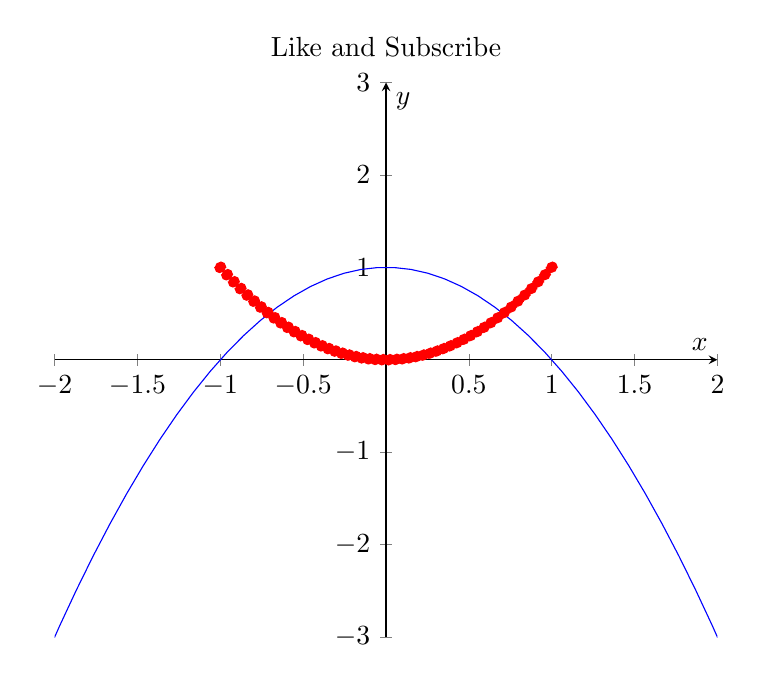
\begin{tikzpicture}
\begin{axis}[
    xmin=-2,xmax=2,ymin=-3,ymax=3,
    axis lines=middle,
    xlabel=$x$,ylabel=$y$,
    title=Like and Subscribe
]
    % 'axis lines' can be set to 'left' or 'middle'
\addplot[color=red,dashed,mark=*,samples=50,domain=-1:1]{x^2}; 
\addplot[color=blue,samples=100]{1-x^2};
\end{axis}
\end{tikzpicture}

\subsection{Sinusoidal}
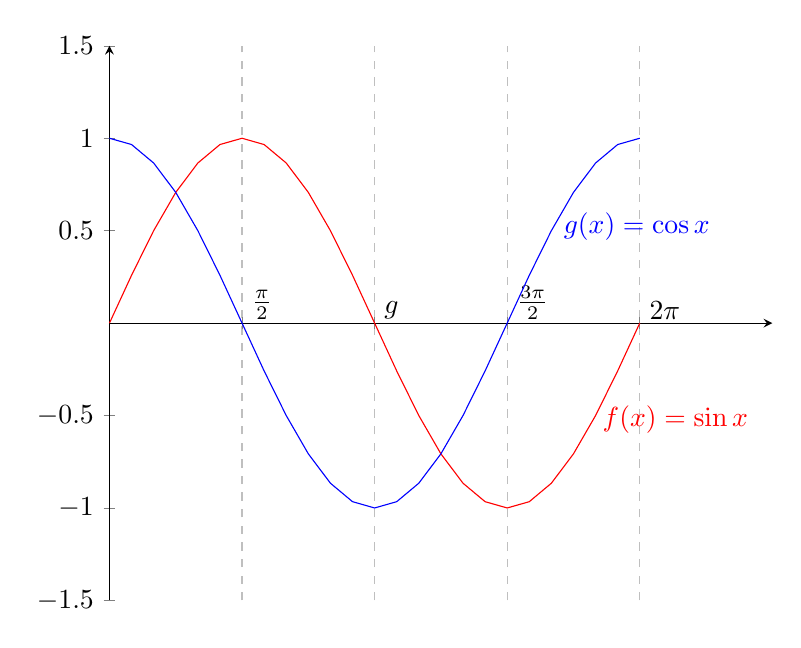
\begin{tikzpicture}
\begin{axis}[clip=false,
    xmin=0,xmax=2.5*pi,
    ymin=-1.5,ymax=1.5,
    axis lines=middle,
    xtick={0,pi/2,pi,3*pi/2,2*pi},
    xticklabels={$0$,$\frac{\pi}{2}$,$g$,$\frac{3\pi}{2}$,$2\pi$},
    xticklabel style={anchor=south west},
    xmajorgrids=true,
    grid style=dashed
    ]
    \addplot[domain=0:2*pi,red]{sin(deg(x))}
    node[right,pos=0.9]{$f(x)=\sin x$};
    % right means text will be to the right side of graph where x=90% mark
    % pos means 90% alonf the x-axis
    \addplot[domain=0:2*pi,blue]{cos(deg(x))}
    node[right,pos=0.85]{$g(x)=\cos x$};
\end{axis}
\end{tikzpicture}


\subsection{Stack Plot : Histogram}
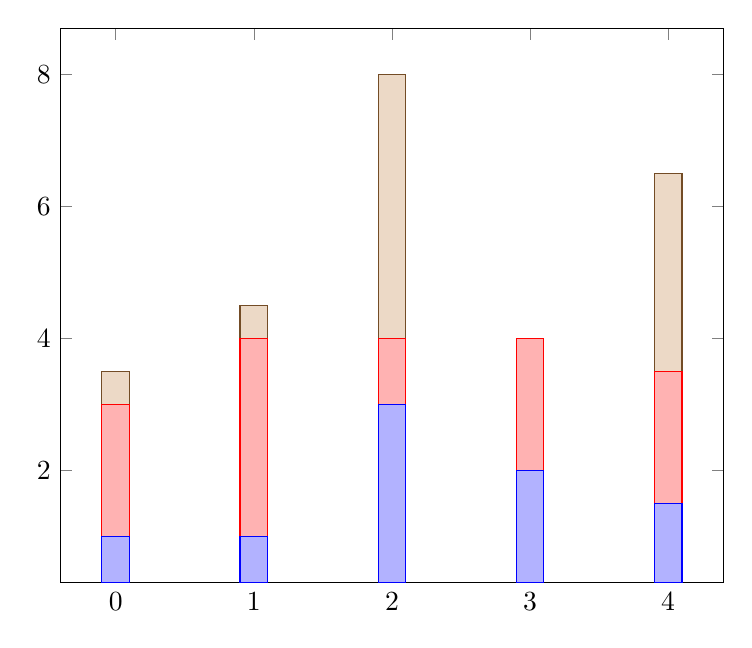
\begin{tikzpicture}
\begin{axis}[ybar stacked]
\addplot coordinates
    {(0,1) (1,1) (2,3) (3,2) (4,1.5)};
\addplot coordinates
    {(0,2) (1,3) (2,1) (3,2) (4,2)};
\addplot coordinates
    {(0,.5) (1,.5) (2,4) (3,0) (4,3)};
    
\end{axis} 
\end{tikzpicture}


\section{3D plot}
\subsection{Ellipsoid}
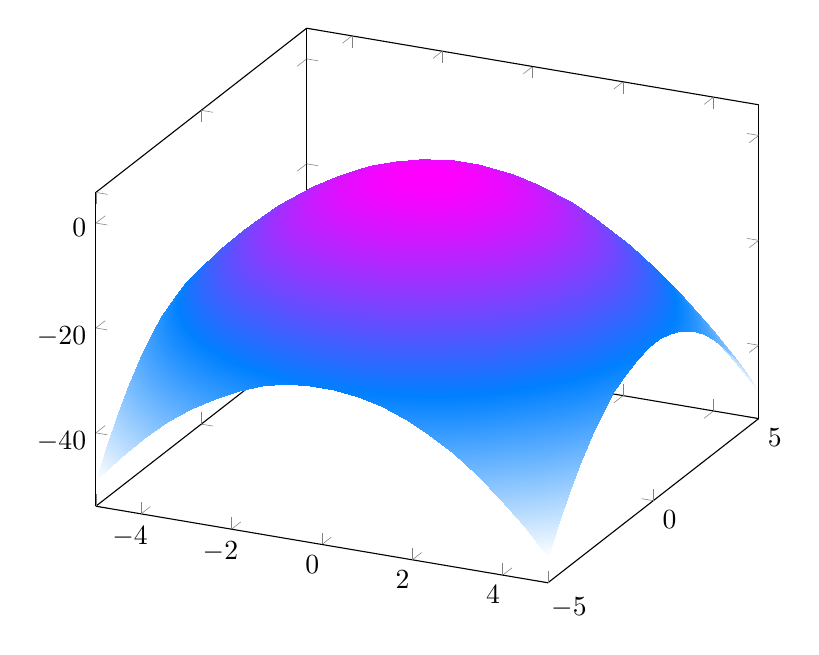
\begin{tikzpicture}
    \begin{axis}[colormap/cool]
        % colormap/cool changes the gradient
       \addplot3[surf,samples=20,shader=interp]{1-x^2-y^2} ;
        % 'surf' can be changed to 'mesh', but remove shader=interp to see full effect
       % shader=interp gets rid of grid lines
   \end{axis}
\end{tikzpicture}


\subsection{Helix}
% Here, x,y,z are function of some variable say t
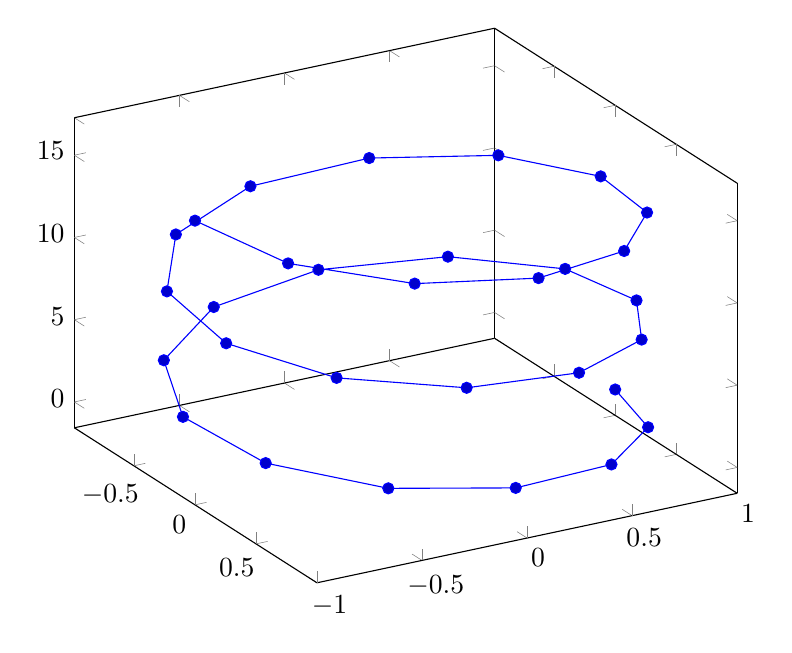
\begin{tikzpicture}
    \begin{axis}[view={60}{30}]
        % view={polar angle}{azimuthal angle}
        \addplot3+[domain=0:5*pi,samples=30,samples y=0]
           ({sin(deg(x))},
           {cos(deg(x))},
           {x});

       % 'samples y=0' gets rid of the line connecting start and endpoints
    \end{axis}
\end{tikzpicture}





\end{document}
